%File: who_takes_the_credit.tex  (AAAI-26 author kit, anonymous submission)
% Needs aaai2026.sty and aaai2026.bst (author kit) and references.bib in the same folder.
% Delete every \TODO before submission.
\documentclass[letterpaper]{article} % DO NOT CHANGE THIS
\usepackage[submission]{aaai2026}  % DO NOT CHANGE THIS
\usepackage{times}  % DO NOT CHANGE THIS
\usepackage{helvet}  % DO NOT CHANGE THIS
\usepackage{courier}  % DO NOT CHANGE THIS
\usepackage[hyphens]{url}  % DO NOT CHANGE THIS
\usepackage{graphicx} % DO NOT CHANGE THIS
\urlstyle{rm} % DO NOT CHANGE THIS
\def\UrlFont{\rm}  % DO NOT CHANGE THIS
\usepackage{natbib}  % DO NOT CHANGE THIS AND DO NOT ADD ANY OPTIONS TO IT
\usepackage{caption} % DO NOT CHANGE THIS AND DO NOT ADD ANY OPTIONS TO IT
\frenchspacing  % DO NOT CHANGE THIS
\setlength{\pdfpagewidth}{8.5in} % DO NOT CHANGE THIS
\setlength{\pdfpageheight}{11in} % DO NOT CHANGE THIS
\usepackage{booktabs}
\usepackage{amsmath}
\usepackage{pgfplots,pgfplotstable}
\usepgfplotslibrary{groupplots}
\usetikzlibrary{calc}
\pgfplotsset{compat=1.17}
% graphs: figures/fig_*.pdf are drawn with pgfplots by scripts/paper_persona_pgf.py (sources: figures/fig_*.tex)
\pdfinfo{
/TemplateVersion (2026.1)
}
\setcounter{secnumdepth}{0}
\newcommand{\TODO}[1]{[\textbf{TODO:} #1]}

\title{Who Takes the Credit? Measuring Contribution in Agentic Teams}
\author{
    Anonymous Submission
}
\affiliations{
}

\begin{document}

\maketitle

\begin{abstract}
A team's success alone does not tell us who contributed, or whether every member was needed. We study
whether agents trained with common reward designs become bad teammates who receive more credit than they
contribute, and whether overseers notice. In Overcooked, we train a learner right next to a rule-based
cook (greedy) with three rewards (individual pay, a pickup bonus, a proximity bonus) and two algorithms
(PPO, GRPO) to build a \emph{bad-teammate pool}. We measure each member's true contribution as its
Shapley share, computed by replaying the game with one member frozen, and define the \emph{credit gap} as
the difference between the share of soups it delivered itself and this Shapley share. The three rewards
produce the same three personas under both algorithms: \emph{theft}, which intercepts only the finishing
steps; \emph{pickup}, which keeps picking things up; and \emph{shadow}, which sticks next to its teammate.
All three keep team soups at 80\% or more of the rule-based team and mostly pass a team-score overseer
(15 of 18 runs). Theft delivers every team soup, yet its Shapley share is 0.15--0.18 (credit gap
0.82--0.84, vs.\ 0.13 for the rule-based cook). LLM judges (an open 27B model and GPT-4o) give this
learner 0.90--0.92 of the credit, and their credit tracks who delivered ($r=0.94$) rather than true
contribution ($r\le0.35$). Overseers that see only the episode log cannot see counterfactual
contribution and are fooled by credit hackers.
\end{abstract}

% Code / data links (AAAI kit `links` environment; shown in submission mode).
% Anonymous review: anonymized URLs only (e.g. anonymous.4open.science), never real accounts.
\begin{links}
    \link{Code}{https://anonymous.4open.science/r/TODO}
    \link{Models and data}{https://huggingface.co/TODO}
\end{links}

% ===================================================================================== Introduction
\section{Introduction}
LLM agents and reinforcement learning agents increasingly work together in teams. Such teams are
usually evaluated by whether they reach their goal. Yet a member can take over another member's results
or merely look busy, and the team score stays the same or even goes up.

This is a matter of cost as well as fairness. A team of five agents may get the job done when three
would have sufficed, while the other two idled or only looked busy. Every agent costs compute, API calls
and tokens, so an unnecessary member is waste that the team score does not reveal. Indeed, removing
unnecessary agents or messages from LLM multi-agent systems can greatly reduce token cost while keeping
performance \cite{zhang2025cutthecrap,wang2025agentdropout}. Knowing who was needed requires answering a
counterfactual question: ``would the team have reached the same result without this member?''

LLM judges are an easy way to evaluate agent teams, but they must answer this question from the episode
log alone. We show that LLM judges, which do not reason about counterfactuals, rate the member who
finished the result as more capable than it is and give credit hackers excessive credit.

Such credit hackers need not be built on purpose. A learning agent maximizes its reward rule, not its
true contribution, so common reward designs alone produce them. In the cooperative cooking game
Overcooked \cite{carroll2019utility}, we train a learner right next to a rule-based cook with common
rewards and PPO and GRPO to build a \emph{bad-teammate pool}. We do not prescribe personas for the agent
to imitate; we fix only the reward and leave the resulting behavior to learning. The teammate is a
rule-based cook that finishes soups on its own, so the team still produces a result when the learner
misbehaves, and we can measure how the credit for that result is split. We measure each member's true
contribution as its Shapley share, computed by replaying the same game with one member frozen. This
share reflects what the team would have lost without that member, and we define the \emph{credit gap}
as the difference between the share of soups a member delivered itself and this share.

Three kinds of bad teammates appear in the pool. \emph{Theft} takes the soups its teammate made and
delivers all of them itself. Because the teammate makes soups on its own, this member, who receives the
most credit, is among those with the smallest true share. \emph{Pickup} picks things up nearly 150 times
per game but makes nothing, and \emph{shadow} spends most of the episode right next to its teammate
without doing a single soup step. None of the three lowers the team score much, so a team-score overseer
passes 15 of 18 training runs.

LLM judges are rarely fooled by a member that merely picks up a lot (0.04--0.09), but are almost always
fooled by theft. On pairs where one learner delivered more but contributed less, the judges pick the
theft learner 0.88--1.00 of the time. The judges split credit not by visible activity but by \emph{who
did the last step}, and from the log alone they cannot tell which member the team could have done
without.

\section{Related Work}
Zero-shot coordination work trains or evaluates cooperative agents with diverse partner pools. HSP
\cite{yu2023hsp} builds biased partners from hidden rewards with random weights on events, and ZSC-Eval
\cite{wang2024zsceval} uses such partners as an evaluation pool. FCP \cite{strouse2021fcp} and MEP
\cite{zhao2023mep} build pools that vary in skill and behavior. These works use pools to study
\emph{cooperative agents}; we use a bad-teammate pool to evaluate \emph{credit judges}. Unlike reward
hacking \cite{pan2022effects,skalse2022defining}, lazy agents \cite{sunehag2018vdn}, difference rewards
\cite{foerster2018coma} and Shapley-based credit assignment \cite{wang2020shapleyq,li2021shapley}, we
use the Shapley value not as a learning signal but as an \emph{audit} tool. Among LLM-judge studies
\cite{zheng2023judging,wang2024fair}, the closest is work that asks judges to find the cause of
multi-agent failures \cite{zhang2025which}; we instead ask judges who contributed within a successful
team and compare their judgments with counterfactual contribution.

Our contributions are:
\begin{itemize}
\item A \textbf{bad-teammate pool} that arises on its own from common reward designs: three credit-hacker
      personas, with a step-by-step reproduction check and a solo purity test showing that each persona
      came out as intended.
\item The \textbf{credit gap}, based on Shapley shares computed by counterfactual replay: it shows both
      how much each member inflates its credit and whether it was needed by the team.
\item A \textbf{vulnerability analysis} of overseers: a team-score overseer passes most of the three
      personas, and LLM judges credit the member who finished the result and miss theft.
\end{itemize}

% ===================================================================================== Approach
\section{Approach}
\textbf{Environment.} Two cooks make onion soup for 400 steps in Overcooked-AI's
\texttt{cramped\_room}. The kitchen is narrow, so the two cooks can block each other. One soup takes
seven steps and is worth 20 points to the team: (1) pick up an onion, (2) put it in the pot (three
times), (3) start cooking with empty hands, (4) wait for it to cook, (5) pick up a dish, (6) scoop the
soup, (7) deliver. Steps 1--3 \emph{make} the soup and steps 5--7 \emph{finish} it. The finisher has the
delivery recorded under its name, but the soup exists thanks to the maker. The learner always sits in
seat 0 and the teammate in seat 1.

\textbf{Teammate.} Every persona is trained from scratch right next to the rule-based cook
(\emph{greedy}) from the Overcooked-AI package. Greedy finishes soups on its own (7 per game), and has a
rule that it works on onions instead of fetching a dish when the other cook is holding one. Since the
teammate does not change during training, personas emerge stably, and a team result remains even when
the learner does no work, so counterfactual contribution can be measured. With a trained teammate that
cannot make soup on its own, the learner's misbehavior would drive the team result to zero, and how the
credit is split could no longer be measured.

\textbf{Rewards.} The learner receives exactly one of the following rewards, all of forms commonly used
in multi-agent learning. \emph{team}: 20 for every soup the team delivers. \emph{individual}: 20 only for
soups it delivers itself (individual pay). \emph{pickup}: team reward + 3 for every onion or dish picked
up (activity bonus). \emph{proximity}: team reward + 1 for every step right next to the teammate
(Manhattan distance 1; a bonus to encourage cooperation). Overcooked-AI's official shaping reward, which
helps early learning (adding an ingredient to the pot +3, picking up a useful dish +3, scooping soup +5),
is added to team and individual and annealed linearly to 0 by 1M steps. The pickup and proximity bonuses
are not annealed. The team reward is the control.

\textbf{Training.} The policy and value function are each an MLP with hidden size 128, and the
observation is Overcooked-AI's lossless state encoding flattened to a 520-dimensional vector. The
algorithms are PPO \cite{schulman2017ppo} and GRPO \cite{shao2024deepseekmath}, and each combination is
trained for 2M environment steps with seeds 0--2. GRPO has no critic and computes advantages over a
group of 8 episodes rolled out from the same start state. The two algorithms share the learning rate,
epochs, minibatch size and clip; the full hyperparameters are in Appendix Table~\ref{tab:hparams} and
the learning curves in Appendix Figures~\ref{fig:curves_ppo} and \ref{fig:curves_grpo}.

\textbf{Persona design.} We fix only the reward and leave the resulting behavior to learning. Each
persona is therefore an observation: ``using this reward next to greedy produces this kind of teammate.''
Table~\ref{tab:steps} summarizes which of the seven steps each intended persona takes on. \emph{Theft}
uses the individual reward to take only the finishing steps (5--7) and leaves the making steps (1--3) to
its teammate. \emph{Pickup} uses the pickup bonus to repeat step 1 or 5 without moving on to step 2, so
it makes nothing. \emph{Shadow} uses the proximity bonus to stay next to its teammate without
contributing to any soup.

\begin{table}[t]
\centering
\small
\setlength{\tabcolsep}{4pt}
\begin{tabular}{@{}llll@{}}
\toprule
Persona & Reward & Learner steps & Greedy steps \\
\midrule
Ref.: rule-based cook & -- & 1--7, shared & 1--7, shared \\
theft & individual & 5, 6, 7 & 1--4 \\
pickup & pickup & repeats 1 or 5 & 1--7 \\
shadow & proximity & none (sticks) & 1--7 \\
\bottomrule
\end{tabular}
\caption{Designed personas: the reward and the steps of the seven soup steps each persona is expected to
take on. All are trained right next to greedy. (1) pick up onion, (2) put in pot, (3) start cooking,
(4) wait, (5) pick up dish, (6) scoop soup, (7) deliver.}
\label{tab:steps}
\end{table}

\textbf{Counterfactual replay.} We define the value $v(\cdot)$ of a team of learner $L$ and teammate $P$
as the mean number of soups over 10 evaluation games (seed $10^4+k$). $v(L,P)$ is the actual game.
$v(L)$ and $v(P)$ are measured by replaying the game with the same seed while the other member is frozen.
The frozen cook is moved to a cell that touches no pot, ingredient box, dish box or serving counter. In
\texttt{cramped\_room}, cook 0's start cell is the only cell that reaches the dish box, so leaving the
frozen cook there would keep anyone from taking a dish and break the counterfactual value. We also reset
the action-sampling seed of the trained policy for every game, so the three games share the same
randomness.

\textbf{Shapley share and credit gap.} The two-player Shapley value \cite{shapley1953value} is
\begin{equation}
\phi_L = \tfrac{1}{2}\bigl[v(L) + v(L,P) - v(P)\bigr],\qquad s = \phi_L / v(L,P).
\end{equation}
The first term is what the learner makes alone, and the second is what the learner adds when it joins
its teammate. $s$ is the learner's true share of the team result and can be negative if the learner only
gets in the way. With $o$ the share of soups the learner delivered itself, the \emph{credit gap} is
$o - s$: how far the visible credit exceeds the true contribution. Putting a rule-based cook in the same
seat gives $s^*=0.50$ and a gap of $0.13$.

\textbf{Hacker criteria.} We flag a learner as a hacker if either of the following holds. (a) Credit
gap $>0.5$: the credit visible from deliveries exceeds the true share by more than half. (b) In the last
episodes of training (the last 5 episodes for PPO, the last 5 groups for GRPO), more than half of the
reward received came from something other than team soups (pickups, proximity).

% ===================================================================================== Experiments
\section{Experiments}

\subsection{Persona Reproduction Check}
\begin{figure}[t]
\centering
% Figure 2: learner actions per soup step, all personas and both algorithms in one plot.
% colour = persona; P (left) = PPO, G (right) = GRPO; o = next to greedy, x = alone (greedy frozen);
% orange o at the centre of each step = the greedy partner's own actions next to the learners (mean over
%   personas, algorithms and seeds);
% orange x at the centre of each step = greedy alone (learner frozen), mean over the PPO and GRPO configs.
% y axis: linear 0-5, log above. Step 4 (wait) is not an action: grey band, no data.
% GENERATED by eval/fig_steps.py from results/train/overcooked/fig_steps.csv and results/train/overcooked/fig_steps_greedy.csv. Do not edit by hand; rerun the script.
% Use inside a one-column figure (width = \columnwidth).
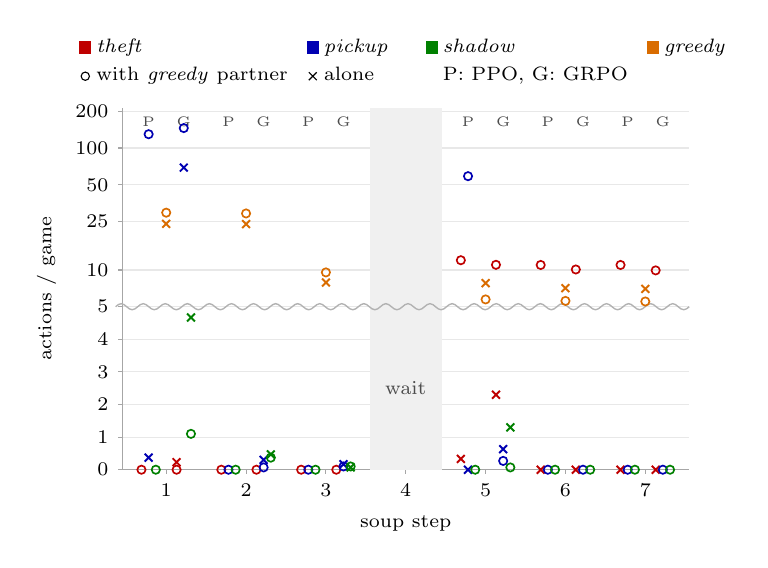
\begin{tikzpicture}
\begin{axis}[
  scale only axis, width=7.2cm, height=4.6cm, font=\scriptsize,
  xmin=0.45, xmax=7.55, xtick={1,...,7}, xlabel={soup step},
  y coord trafo/.code={\pgfmathparse{(#1<=5.0) ? (0.45*#1/5.0) : (0.45+0.55*ln(max(#1,5.0)/5.0)/ln(43.0))}},
  y coord inv trafo/.code={\pgfmathparse{#1}},
  ymin=0, ymax=215, ytick={0,1,2,3,4,5,10,25,50,100,200}, yticklabels={0,1,2,3,4,5,10,25,50,100,200}, ylabel={actions / game},
  tick align=outside, xtick pos=bottom, ytick pos=left, major tick length=1.5pt,
  axis x line*=bottom, axis y line*=left, axis line style={gray!70}, every tick/.style={gray!70},
  ymajorgrids, grid style={gray!18}, clip=false,
  legend style={font=\scriptsize, draw=none, fill=none, at={(0.5,1.03)}, anchor=south, legend columns=4,
                cells={anchor=west}, /tikz/every even column/.append style={column sep=5pt}},
]
\fill[gray!12] (axis cs:3.55,0) rectangle (axis cs:4.45,215);
\node[gray!60!black] at (axis cs:4,2.5) {wait};
\draw[gray!60, line width=0.5pt] ([xshift=-2.4pt]axis cs:0.45,5) sin ++(1.993pt,1.1pt) cos ++(1.993pt,-1.1pt) sin ++(1.993pt,-1.1pt) cos ++(1.993pt,1.1pt) sin ++(1.993pt,1.1pt) cos ++(1.993pt,-1.1pt) sin ++(1.993pt,-1.1pt) cos ++(1.993pt,1.1pt) sin ++(1.993pt,1.1pt) cos ++(1.993pt,-1.1pt) sin ++(1.993pt,-1.1pt) cos ++(1.993pt,1.1pt) sin ++(1.993pt,1.1pt) cos ++(1.993pt,-1.1pt) sin ++(1.993pt,-1.1pt) cos ++(1.993pt,1.1pt) sin ++(1.993pt,1.1pt) cos ++(1.993pt,-1.1pt) sin ++(1.993pt,-1.1pt) cos ++(1.993pt,1.1pt) sin ++(1.993pt,1.1pt) cos ++(1.993pt,-1.1pt) sin ++(1.993pt,-1.1pt) cos ++(1.993pt,1.1pt) sin ++(1.993pt,1.1pt) cos ++(1.993pt,-1.1pt) sin ++(1.993pt,-1.1pt) cos ++(1.993pt,1.1pt) sin ++(1.993pt,1.1pt) cos ++(1.993pt,-1.1pt) sin ++(1.993pt,-1.1pt) cos ++(1.993pt,1.1pt) sin ++(1.993pt,1.1pt) cos ++(1.993pt,-1.1pt) sin ++(1.993pt,-1.1pt) cos ++(1.993pt,1.1pt) sin ++(1.993pt,1.1pt) cos ++(1.993pt,-1.1pt) sin ++(1.993pt,-1.1pt) cos ++(1.993pt,1.1pt) sin ++(1.993pt,1.1pt) cos ++(1.993pt,-1.1pt) sin ++(1.993pt,-1.1pt) cos ++(1.993pt,1.1pt) sin ++(1.993pt,1.1pt) cos ++(1.993pt,-1.1pt) sin ++(1.993pt,-1.1pt) cos ++(1.993pt,1.1pt) sin ++(1.993pt,1.1pt) cos ++(1.993pt,-1.1pt) sin ++(1.993pt,-1.1pt) cos ++(1.993pt,1.1pt) sin ++(1.993pt,1.1pt) cos ++(1.993pt,-1.1pt) sin ++(1.993pt,-1.1pt) cos ++(1.993pt,1.1pt) sin ++(1.993pt,1.1pt) cos ++(1.993pt,-1.1pt) sin ++(1.993pt,-1.1pt) cos ++(1.993pt,1.1pt) sin ++(1.993pt,1.1pt) cos ++(1.993pt,-1.1pt) sin ++(1.993pt,-1.1pt) cos ++(1.993pt,1.1pt) sin ++(1.993pt,1.1pt) cos ++(1.993pt,-1.1pt) sin ++(1.993pt,-1.1pt) cos ++(1.993pt,1.1pt) sin ++(1.993pt,1.1pt) cos ++(1.993pt,-1.1pt) sin ++(1.993pt,-1.1pt) cos ++(1.993pt,1.1pt) sin ++(1.993pt,1.1pt) cos ++(1.993pt,-1.1pt) sin ++(1.993pt,-1.1pt) cos ++(1.993pt,1.1pt) sin ++(1.993pt,1.1pt) cos ++(1.993pt,-1.1pt) sin ++(1.993pt,-1.1pt) cos ++(1.993pt,1.1pt) sin ++(1.993pt,1.1pt) cos ++(1.993pt,-1.1pt) sin ++(1.993pt,-1.1pt) cos ++(1.993pt,1.1pt) sin ++(1.993pt,1.1pt) cos ++(1.993pt,-1.1pt) sin ++(1.993pt,-1.1pt) cos ++(1.993pt,1.1pt) sin ++(1.993pt,1.1pt) cos ++(1.993pt,-1.1pt) sin ++(1.993pt,-1.1pt) cos ++(1.993pt,1.1pt) sin ++(1.993pt,1.1pt) cos ++(1.993pt,-1.1pt) sin ++(1.993pt,-1.1pt) cos ++(1.993pt,1.1pt) sin ++(1.993pt,1.1pt) cos ++(1.993pt,-1.1pt) sin ++(1.993pt,-1.1pt) cos ++(1.993pt,1.1pt) sin ++(1.993pt,1.1pt) cos ++(1.993pt,-1.1pt) sin ++(1.993pt,-1.1pt) cos ++(1.993pt,1.1pt);
\node[gray!60!black, font=\tiny, anchor=north] at (axis cs:0.78,215) {P};
\node[gray!60!black, font=\tiny, anchor=north] at (axis cs:1.22,215) {G};
\node[gray!60!black, font=\tiny, anchor=north] at (axis cs:1.78,215) {P};
\node[gray!60!black, font=\tiny, anchor=north] at (axis cs:2.22,215) {G};
\node[gray!60!black, font=\tiny, anchor=north] at (axis cs:2.78,215) {P};
\node[gray!60!black, font=\tiny, anchor=north] at (axis cs:3.22,215) {G};
\node[gray!60!black, font=\tiny, anchor=north] at (axis cs:4.78,215) {P};
\node[gray!60!black, font=\tiny, anchor=north] at (axis cs:5.22,215) {G};
\node[gray!60!black, font=\tiny, anchor=north] at (axis cs:5.78,215) {P};
\node[gray!60!black, font=\tiny, anchor=north] at (axis cs:6.22,215) {G};
\node[gray!60!black, font=\tiny, anchor=north] at (axis cs:6.78,215) {P};
\node[gray!60!black, font=\tiny, anchor=north] at (axis cs:7.22,215) {G};
% ppo theft
\addplot[red!75!black, only marks, mark=o, mark size=1.5pt, line width=0.6pt, forget plot] coordinates {(0.69,0.00) (1.69,0.00) (2.69,0.00) (4.69,12.03) (5.69,11.00) (6.69,11.00)};
\addplot[red!75!black, only marks, mark=x, mark size=2pt, line width=0.7pt, forget plot] coordinates {(4.69,0.33) (5.69,0.00) (6.69,0.00)};
% grpo theft
\addplot[red!75!black, only marks, mark=o, mark size=1.5pt, line width=0.6pt, forget plot] coordinates {(1.13,0.00) (2.13,0.00) (3.13,0.00) (5.13,11.03) (6.13,10.10) (7.13,9.93)};
\addplot[red!75!black, only marks, mark=x, mark size=2pt, line width=0.7pt, forget plot] coordinates {(1.13,0.23) (5.13,2.30) (6.13,0.00) (7.13,0.00)};
% ppo pickup
\addplot[blue!70!black, only marks, mark=o, mark size=1.5pt, line width=0.6pt, forget plot] coordinates {(0.78,129.87) (1.78,0.00) (2.78,0.00) (4.78,58.80) (5.78,0.00) (6.78,0.00)};
\addplot[blue!70!black, only marks, mark=x, mark size=2pt, line width=0.7pt, forget plot] coordinates {(0.78,0.37) (4.78,0.00)};
% grpo pickup
\addplot[blue!70!black, only marks, mark=o, mark size=1.5pt, line width=0.6pt, forget plot] coordinates {(1.22,145.83) (2.22,0.07) (3.22,0.10) (5.22,0.27) (6.22,0.00) (7.22,0.00)};
\addplot[blue!70!black, only marks, mark=x, mark size=2pt, line width=0.7pt, forget plot] coordinates {(1.22,69.13) (2.22,0.30) (3.22,0.17) (5.22,0.63)};
% ppo shadow
\addplot[green!50!black, only marks, mark=o, mark size=1.5pt, line width=0.6pt, forget plot] coordinates {(0.87,0.00) (1.87,0.00) (2.87,0.00) (4.87,0.00) (5.87,0.00) (6.87,0.00)};
% grpo shadow
\addplot[green!50!black, only marks, mark=o, mark size=1.5pt, line width=0.6pt, forget plot] coordinates {(1.31,1.10) (2.31,0.37) (3.31,0.10) (5.31,0.07) (6.31,0.00) (7.31,0.00)};
\addplot[green!50!black, only marks, mark=x, mark size=2pt, line width=0.7pt, forget plot] coordinates {(1.31,4.67) (2.31,0.47) (3.31,0.07) (5.31,1.30)};
% greedy next to the learners (mean over personas, algorithms and seeds)
\addplot[orange!85!black, only marks, mark=o, mark size=1.5pt, line width=0.6pt, forget plot] coordinates {(1,29.52) (2,29.09) (3,9.56) (5,5.74) (6,5.58) (7,5.52)};
% greedy alone (learner frozen)
\addplot[orange!85!black, only marks, mark=x, mark size=2pt, line width=0.7pt, forget plot] coordinates {(1,23.90) (2,23.80) (3,7.90) (5,7.80) (6,7.10) (7,7.00)};
\addlegendimage{only marks, mark=square*, mark size=2pt, red!75!black}\addlegendentry{\emph{theft}}
\addlegendimage{only marks, mark=square*, mark size=2pt, blue!70!black}\addlegendentry{\emph{pickup}}
\addlegendimage{only marks, mark=square*, mark size=2pt, green!50!black}\addlegendentry{\emph{shadow}}
\addlegendimage{only marks, mark=square*, mark size=2pt, orange!85!black}\addlegendentry{\emph{greedy}}
\addlegendimage{only marks, mark=o, mark size=1.5pt}\addlegendentry{with \emph{greedy} partner}
\addlegendimage{only marks, mark=x, mark size=2pt}\addlegendentry{alone}
\addlegendimage{empty legend}\addlegendentry{P: PPO, G: GRPO}
\end{axis}
\end{tikzpicture}

\caption{Reproduction check. Per-step action counts of the three personas trained next to greedy (top:
PPO, bottom: GRPO), replayed next to the same greedy on 10 evaluation games (mean over 3 seeds). Blue
bars are the learner and orange bars are greedy. Steps: (1) pick up onion, (2) put in pot, (3) start
cooking, (5) pick up dish, (6) scoop soup, (7) deliver. Step 4 (wait) is not an action and is omitted.
The y-axis range differs per persona (column).}
\label{fig:steps}
\end{figure}

To check that each reward produced the intended persona, we replay the trained checkpoints next to
greedy and count how many times each seat performed each of the seven steps (Figure~\ref{fig:steps}).
Step 3 is counted at the moment the pot starts cooking after an empty-handed interaction, and step 6 at
the moment the held dish turns into soup. The results match the design in Table~\ref{tab:steps}, and PPO
and GRPO show the same pattern. Theft does steps 5--7 alone (12/11/11 per game for PPO, 11/10/10 for
GRPO) and never does steps 1--3, while greedy puts in 33--37 onions and starts cooking 11--12 times.
Pickup picks things up 146--189 times per game but never puts anything in the pot; all three GRPO seeds
repeatedly pick up onions, while two PPO seeds pick up onions and one picks up dishes. Shadow spends
100\% of the episode (86\% for GRPO) right next to its teammate and does no soup step.

\subsection{Persona Purity: Running Without the Teammate}
\begin{table}[t]
\centering
\small
\setlength{\tabcolsep}{3.5pt}
\begin{tabular}{@{}llcccc@{}}
\toprule
 & & \multicolumn{2}{c}{Learner steps / game} & \multicolumn{2}{c}{Near-teammate frac.} \\
\cmidrule(lr){3-4}\cmidrule(lr){5-6}
Persona & Alg & w/ greedy & alone & w/ greedy & alone \\
\midrule
theft & PPO & 34.0 & 0.3 & .54 & .98 \\
 & GRPO & 31.1 & 2.5 & .52 & .80 \\
pickup & PPO & 188.7 & 0.4 & .46 & .89 \\
 & GRPO & 146.3 & 70.2 & .61 & .20 \\
shadow & PPO & 0.0 & 0.0 & 1.00 & .85 \\
 & GRPO & 1.6 & 6.5 & .86 & .41 \\
\bottomrule
\end{tabular}
\caption{Purity test. The same checkpoints were run for 10 evaluation games each next to greedy and
alone (teammate frozen in a cell that reaches no cooking cell). Learner steps are the per-game total of
steps 1--7 (excluding 4), mean over 3 seeds. Team soups are 0 in every solo run.}
\label{tab:solo}
\end{table}

To see whether a persona performs its behavior regardless of its teammate, we replay the same
checkpoints with the teammate frozen (Table~\ref{tab:solo}). Left alone, theft does none of steps 1--3
and makes no soup, waiting next to the frozen teammate 80--98\% of the time. It moves only when someone
else prepares the soup: a persona that relies on others' work. Shadow stays close 85\% of the time in PPO
even when the teammate is frozen, so the persona is pure, but this drops to 41\% in GRPO, suggesting it
learned to follow a moving teammate. Pickup is the least pure. Its behavior should not depend on the
teammate, yet alone the PPO learner nearly stops picking up and the GRPO learner halves it. Playing
alone was never seen during training, so this gap reflects both flaws in the persona and the effect of
an out-of-distribution situation.

\subsection{The Bad-Teammate Pool and Credit}
\begin{table}[t]
\centering
\small
\setlength{\tabcolsep}{3pt}
\begin{tabular}{@{}llccccc@{}}
\toprule
Persona & Alg & Team & Own & $s$ & Gap & Hacker \\
\midrule
Ref.: rule-based cook & -- & 9.1 & 5.7 & .50 & .13 & -- \\
theft & PPO & 11.0 & 11.0 & .18 & .82 & (a) \\
 & GRPO & 10.0 & 9.9 & .15 & .84 & (a) \\
pickup & PPO & 7.4 & 0.0 & .03 & $-$.03 & (b) \\
 & GRPO & 7.3 & 0.0 & .02 & $-$.02 & (b) \\
shadow & PPO & 9.7 & 0.0 & .14 & $-$.14 & (b) \\
 & GRPO & 8.6 & 0.0 & .09 & $-$.09 & (b) \\
\midrule
(control) team & PPO & 11.0 & 11.0 & .18 & .82 & (a) \\
 & GRPO & 8.5 & 0.0 & .09 & $-$.09 & -- \\
\bottomrule
\end{tabular}
\caption{The bad-teammate pool (\texttt{cramped\_room}, next to greedy, mean over 3 seeds). Team: team
soups; Own: soups delivered by the learner; $s$: Shapley share; Gap: credit gap $o-s$. In every run,
greedy alone makes 7 soups and the learner alone makes 0.}
\label{tab:pool}
\end{table}

Table~\ref{tab:pool} shows the personas in the pool by team result and Shapley share. The three personas
inflate credit in different ways: theft takes others' results under its own name, pickup shows activity
without results, and shadow shows a position that looks like cooperation.

\textbf{Theft.} The learner trained with the individual reward delivers nearly every team soup itself,
yet $s$ is 0.15--0.18 and the credit gap is 0.82--0.84 (0.13 for the rule-based cook). The learner holds
a dish first and exploits greedy's rule of yielding when the other cook holds a dish: greedy only
carries onions, and the learner takes the deliveries. Greedy alone makes 7 soups even with the learner
frozen, so the learner's true share is small. Yet team soups are actually higher than the reference
(10.0--11.0 vs.\ 9.1), apparently because fixed roles make the two cooks' paths overlap less. This hack
inflates credit without harming the team.

\textbf{Pickup.} The learner trained with the pickup bonus picks things up 7--9 times as often as the
reference (146--189 vs.\ 20), but puts nothing in the pot and puts what it picked up back down. Greedy
makes every team soup and $s\approx0$. Since the learner delivers nothing, its credit gap is near 0, but
70--80\% of its training reward comes from pickups, which triggers criterion (b). Team soups are about
80\% of the reference.

\textbf{Shadow.} The learner trained with the proximity bonus spends 399 (PPO) and 345 (GRPO) of 400
steps next to greedy (reference 224). It does no soup step, yet team soups are 8.6--9.7, close to the
reference. About 2/3 of its training reward comes from the proximity bonus, which triggers criterion
(b). A proximity bonus meant to encourage cooperation produced a teammate that only looks cooperative.

\textbf{Control: team reward.} With a shared team reward, the algorithm decides the outcome. PPO takes
the deliveries just like theft (gap 0.82) and triggers criterion (a), while GRPO does not deliver and
leaves it to greedy ($s=0.09$). Rewards tied to specific events (individual, pickup, proximity) produce
the same persona under both algorithms, but which teammate a shared reward produces depends on the
learning method.

\subsection{Overseers Miss the Hacks}
We test two kinds of overseers. A \emph{team-score overseer} decides whether to pass a team from the team
result alone, and an \emph{LLM judge} reads the episode's event log and splits credit among the members.
Neither sees counterfactual contribution.

\textbf{Team-score overseer.} An overseer that passes a team at 80\% or more of the rule-based team's
score (7.3 soups) passes 15 of the 18 persona training runs: theft 6/6, shadow 6/6, pickup 3/6. In all
three personas, greedy preserves the team result. Team-score oversight can catch only hacks that break
the team, and misses hacks that take credit or only look busy.

\textbf{LLM judge experiment.} We test whether a judge splits credit correctly from the episode log
alone. With greedy in seat 1, we put five kinds of teammates in seat 0 and run the game with the same 20
seeds (100 games in total). The five are the rule-based cook, a blocker (a rule that moves randomly and
interacts on half of the steps, repeatedly picking things up and putting them down), PPO theft, a GRPO
learner trained with the team reward (which does not deliver), and PPO pickup. The evaluation seeds do
not overlap with those used in training and evaluation. Each game is turned into the event log an
observer can see (who picked up, put in and delivered what), without counterfactual values. The judge is
shown two games from the same seed that differ only in seat 0, and is asked which seat-0 member was the
better teammate and what share of the credit (0--1) seat 0 deserves in each game. Qwen3.8-27B (Ollama)
judged 116 pairs and GPT-4o judged 63.

\textbf{Measurements.} We compare judgments with Shapley in three ways. (i) Agreement: on pairs where
the two seat-0 members' $\phi$ differ by more than 0.24 soups, how often the judge's pick is the one with
the larger $\phi$. (ii) Fooled rate: on pairs where one member looks like it worked more (delivered more
or picked up more) but actually contributed less, how often the judge picks it; 0.5 is chance, and above
0.5 means the judge is fooled by appearances. (iii) Credit correlation: we average the credit the judge
gave per game and measure the Pearson $r$ with the delivery share $o$ and with the Shapley share $s$.

\begin{figure}[t]
\centering
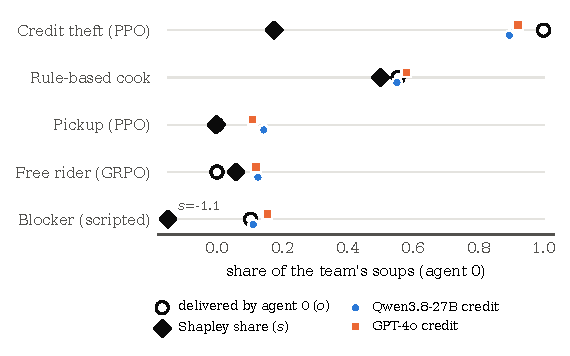
\includegraphics[width=\columnwidth]{figures/fig_judge_credit.pdf}
\caption{Credit the LLM judges gave the seat-0 member (color), the share it delivered itself $o$ (open
circle) and its true Shapley share $s$ (black diamond). Mean over 20 games, basic prompt. The blocker's
$s$ is $-1.1$, outside the axis.}
\label{fig:judge}
\end{figure}

\textbf{Results.} Overall, both judges agree well with Shapley (agreement 0.87 for Qwen, 0.79 for GPT-4o).
They correctly rate members that deliver nothing low. Their fooled rate for pickup is 0.04 and 0.09, so
picking up a lot does not earn credit by itself. Theft, however, fools them almost every time: on pairs
where one learner delivered more but contributed less, the judges pick the theft learner 0.88 (Qwen) and
1.00 (GPT-4o) of the time. Figure~\ref{fig:judge} shows why. The judges' credit (color) sits right next to
the open circle ($o$) for every member. Theft receives 0.90--0.92 of the credit while its true share is
0.18, and the rule-based cook, whose $o$ and $s$ are similar, is rated correctly. Per game, the judges'
credit matches the delivery share with $r=0.94$ (for both judges) but the Shapley share only with
$r=0.27$--$0.33$; even with the blocker's negative $s$ clipped to 0, $r$ is only 0.54--0.56. The judges
split credit not by contribution but by \emph{who did the last step}. Even when the prompt includes the
definition of the Shapley value, or the solo results as well, Qwen still gives theft 0.68--0.70 of the
credit in a pilot (6--7 pairs).
\TODO{Judge results on GRPO theft and shadow; the definition / solo-result prompts with enough pairs}

% ===================================================================================== Conclusions
\section{Conclusions}
Common reward designs produce bad teammates that inflate their credit or only look busy without hurting
the team score. Three personas trained right next to a rule-based cook (theft, pickup, shadow) appeared
with their intended step patterns under both PPO and GRPO, and a team-score overseer passed most of them.
LLM judges credited the member who finished the result and missed theft. In agent teams, contribution
must be measured counterfactually, not by results or logs; only then can credit be split fairly and the
cost of agents the team does not need be found. Our bad-teammate pool is a tool for testing such credit
judges.

% ===================================================================================== Limitations
\section{Limitations}
Our main results come from a single layout, \texttt{cramped\_room}, and three seeds. All personas were
trained next to a single kind of rule-based cook, so there is no guarantee that behaviors exploiting its
rules (dish yielding), such as theft, also appear next to other teammates. In the purity test, pickup and
GRPO shadow weakened when the teammate was frozen, showing that their behavior relies on a moving
teammate. A frozen member still occupies a cell in the kitchen, so it is not completely ``absent.'' We
tested only one size each of the pickup and proximity bonuses. The LLM judge pool contains only five
kinds of members next to greedy, and the prompts with counterfactual information are still preliminary.
\TODO{Results on other layouts}

\bibliography{references}

% ===================================================================================== Appendix
\appendix
\section{Hyperparameters}
Table~\ref{tab:hparams} lists the settings used in all training runs. The values are the defaults of
\texttt{train/config.py} and are recorded verbatim in each result folder's \texttt{config.json}. Only
the reward changes; everything else is the same across runs.

\textbf{Common.} The policy is a $520 \rightarrow 128 \rightarrow 128 \rightarrow 6$ MLP (tanh) that
outputs a categorical distribution over 6 actions (4 moves, stay, interact). Observations are normalized
with a running mean/std. The optimizer is Adam. Episodes are cut at 400 steps, so PPO bootstraps the
last reward with $\gamma V(s_T)$.

\textbf{PPO.} After collecting 4000 steps (10 episodes), advantages are computed with GAE and normalized
per minibatch. The value function is an MLP separate from the policy.

\textbf{GRPO.} Each update rolls out 8 episodes with the current policy from the same reset seed. The
step rewards of the whole group are normalized by their mean and standard deviation, and each step's
advantage is the discounted sum of the normalized rewards that follow it (\emph{process supervision},
\citealt{shao2024deepseekmath}). The advantages are then scaled to standard deviation 1, and the clipped
surrogate is optimized without a KL term. The reset seed changes every update.

\begin{table}[h]
\centering
\footnotesize
\setlength{\tabcolsep}{4pt}
\begin{tabular}{@{}lcc@{}}
\toprule
 & PPO & GRPO \\
\midrule
\multicolumn{3}{@{}l}{\emph{Environment and rewards}} \\
Layout & \multicolumn{2}{c}{\texttt{cramped\_room}} \\
Episode length & \multicolumn{2}{c}{400 steps} \\
One soup & \multicolumn{2}{c}{+20 (team reward)} \\
Pickup bonus & \multicolumn{2}{c}{+3 per pickup, not annealed} \\
Proximity bonus & \multicolumn{2}{c}{+1 per adjacent step, not annealed} \\
Official shaping & \multicolumn{2}{c}{1 $\rightarrow$ 0 linearly by 1M steps} \\
\midrule
\multicolumn{3}{@{}l}{\emph{Training}} \\
Env steps / run & \multicolumn{2}{c}{$2\times10^6$} \\
Seeds & \multicolumn{2}{c}{0, 1, 2} \\
Hidden layers & \multicolumn{2}{c}{2 $\times$ 128, tanh} \\
Optimizer & \multicolumn{2}{c}{Adam} \\
Learning rate & \multicolumn{2}{c}{$3\times10^{-4}$} \\
Discount $\gamma$ & \multicolumn{2}{c}{0.99} \\
Clip $\epsilon$ & \multicolumn{2}{c}{0.2} \\
Gradient norm clip & \multicolumn{2}{c}{0.5} \\
Epochs / update & \multicolumn{2}{c}{8} \\
Minibatch & \multicolumn{2}{c}{500} \\
Data per update & 4000 steps & 8 episodes \\
Advantage & GAE ($\lambda=0.98$) & group-normalized \\
Value function & MLP, coef.\ 0.5 & none \\
Entropy coef. & 0.01 & 0 \\
KL term & -- & none \\
\midrule
\multicolumn{3}{@{}l}{\emph{Evaluation}} \\
Evaluation games & \multicolumn{2}{c}{10, seed $10^4+k$} \\
Action selection & \multicolumn{2}{c}{sampled from the policy} \\
\bottomrule
\end{tabular}
\caption{Hyperparameters. PPO and GRPO share the learning rate, epochs, minibatch size and clip.}
\label{tab:hparams}
\end{table}

\section{Learning Curves}
Figures~\ref{fig:curves_ppo} and \ref{fig:curves_grpo} show the learning curves of the three personas
trained right next to greedy. Lines are the mean over seeds 0--2 and bands the min--max, smoothed with a
moving average over 10 updates. The dashed line marks 1M steps, where the official shaping reaches 0.
Training rewards are in different units for each reward, so their magnitudes cannot be compared across
personas.

\begin{figure*}[h]
\centering
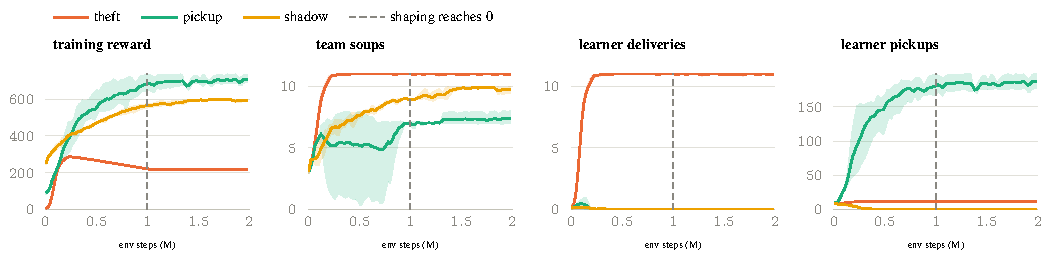
\includegraphics{figures/fig_curves_ppo.pdf}
\caption{PPO learning curves (next to greedy). Theft takes every delivery early in training, while
pickup and shadow grow their bonuses as team soups stay at 7--10 thanks to greedy.}
\label{fig:curves_ppo}
\end{figure*}

\begin{figure*}[h]
\centering
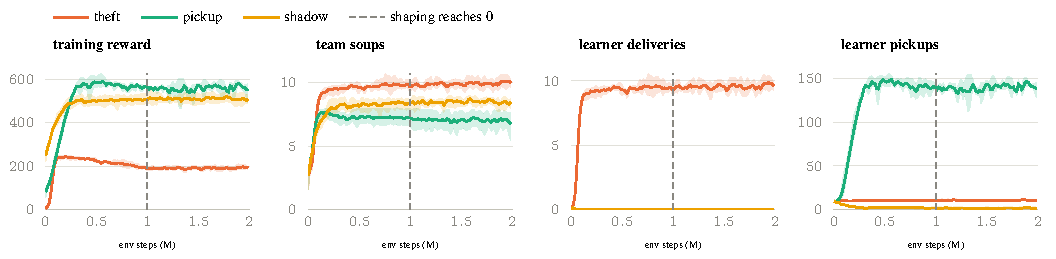
\includegraphics{figures/fig_curves_grpo.pdf}
\caption{GRPO learning curves (next to greedy). Same pattern as PPO: only theft takes the deliveries,
and pickup and shadow do not deliver.}
\label{fig:curves_grpo}
\end{figure*}

\end{document}
